\section{Comparison with existing bounds}\label{sec:bounds}

The expected sensitivity is compared with the published limits on the same benchmark. FASER's limits on the
$(1,1)_{-1}$ fermion with $N_{\rm IC}=2$~\cite{FASER:2026fsy,FASER:HEPData181308v1t2} are an exact model match and are
taken from HEPData; Farina and Low's recasts~\cite[Table~II]{Farina:2017cts} exclude $\mQ<650$ ($150$)$\GeV$ for $E$ and
$\mQ<350$ ($60$)$\GeV$ for $\Etil$ at $\Lam=1\eV$ ($100\eV$) and give no limit at $1\keV$; the D0 exclusion, $\mQ<107\GeV$ for
$\Lam=10\keV$--$1\MeV$~\cite{D0:2010kkd}, is a probable match (the SU(2)$_L$ representation is not stated). The
FASER-rendered heavy-stable-particle and monojet curves differ from Farina and Low's table at two points; the difference is
documented but not resolved (\rep{stage5/EXTERNAL_BOUNDS.md}).
In the $\Lam$ range of our grid ($0.45$--$5\keV$) all these bounds lie at $\mQ\lesssim180\GeV$, below the lightest
mass of the grid. Figure~\ref{fig:excl} shows the expected
$\sigma_{95}/\sigma_{\rm norm}$ of the fallback on the full $(\mQ,\Lam)$ grid of the fermion with the FASER exclusion
overlaid; the other limits fall outside the plotted range and are listed in the caption. No cell is below one (minimum 790 at $200\GeV$,
$1.5\keV$), so no exclusion, $\pm1\sigma$ or discovery contour exists. \textbf{This study therefore adds no exclusion beyond
the existing bounds}; it quantifies how far a barrel-only plane search at pile-up 200, with backgrounds estimated purely from
simulation, is from sensitivity.

\paragraph{Comparison with published reach projections.} Our null result comes from the background method, not from a
tension with Knapen et al.~\cite{Knapen:2017kly} and Li et al.~\cite{Li:2019wce}. With zero background our fallback
efficiencies would exclude $E$ up to $\approx1\TeV$ with $3\abinv$, and give a 5-event reach of $\approx0.6\TeV$ with
$300\fb^{-1}$, close to the $650\GeV$ of Knapen et al.\ (\EST{}, with $f_{200}$; their set-up differs: 2\,T field,
$\sqrt s=13\TeV$, eight-layer ATLAS-like barrel); our total efficiency
($f_{200}A\,\Eff\approx0.005$ at $E$ 500, barrel only) is about four times below theirs. An exclusion at $E$ 200,
$1.5\keV$ would need a total background below $\approx8\times10^2$ events ($\sigma_{\ln}=1$, \EST{}), whereas our estimate
there is a zero-count upper bound of $\sim6\times10^5$ events (median) from 500--2000 simulated events per process, set
by single-interaction topologies (PV pairs, decays in flight, nuclear interactions, loopers) that neither study treated
and by SM terms estimated here at the zero-count level, none of which scales with pile-up. Both studies assumed zero or a
small background after their cuts. We therefore do not
show those projections to be wrong: at pile-up 200 the background-free assumption cannot be confirmed by simulation alone.

\begin{figure}[htbp]
\centering
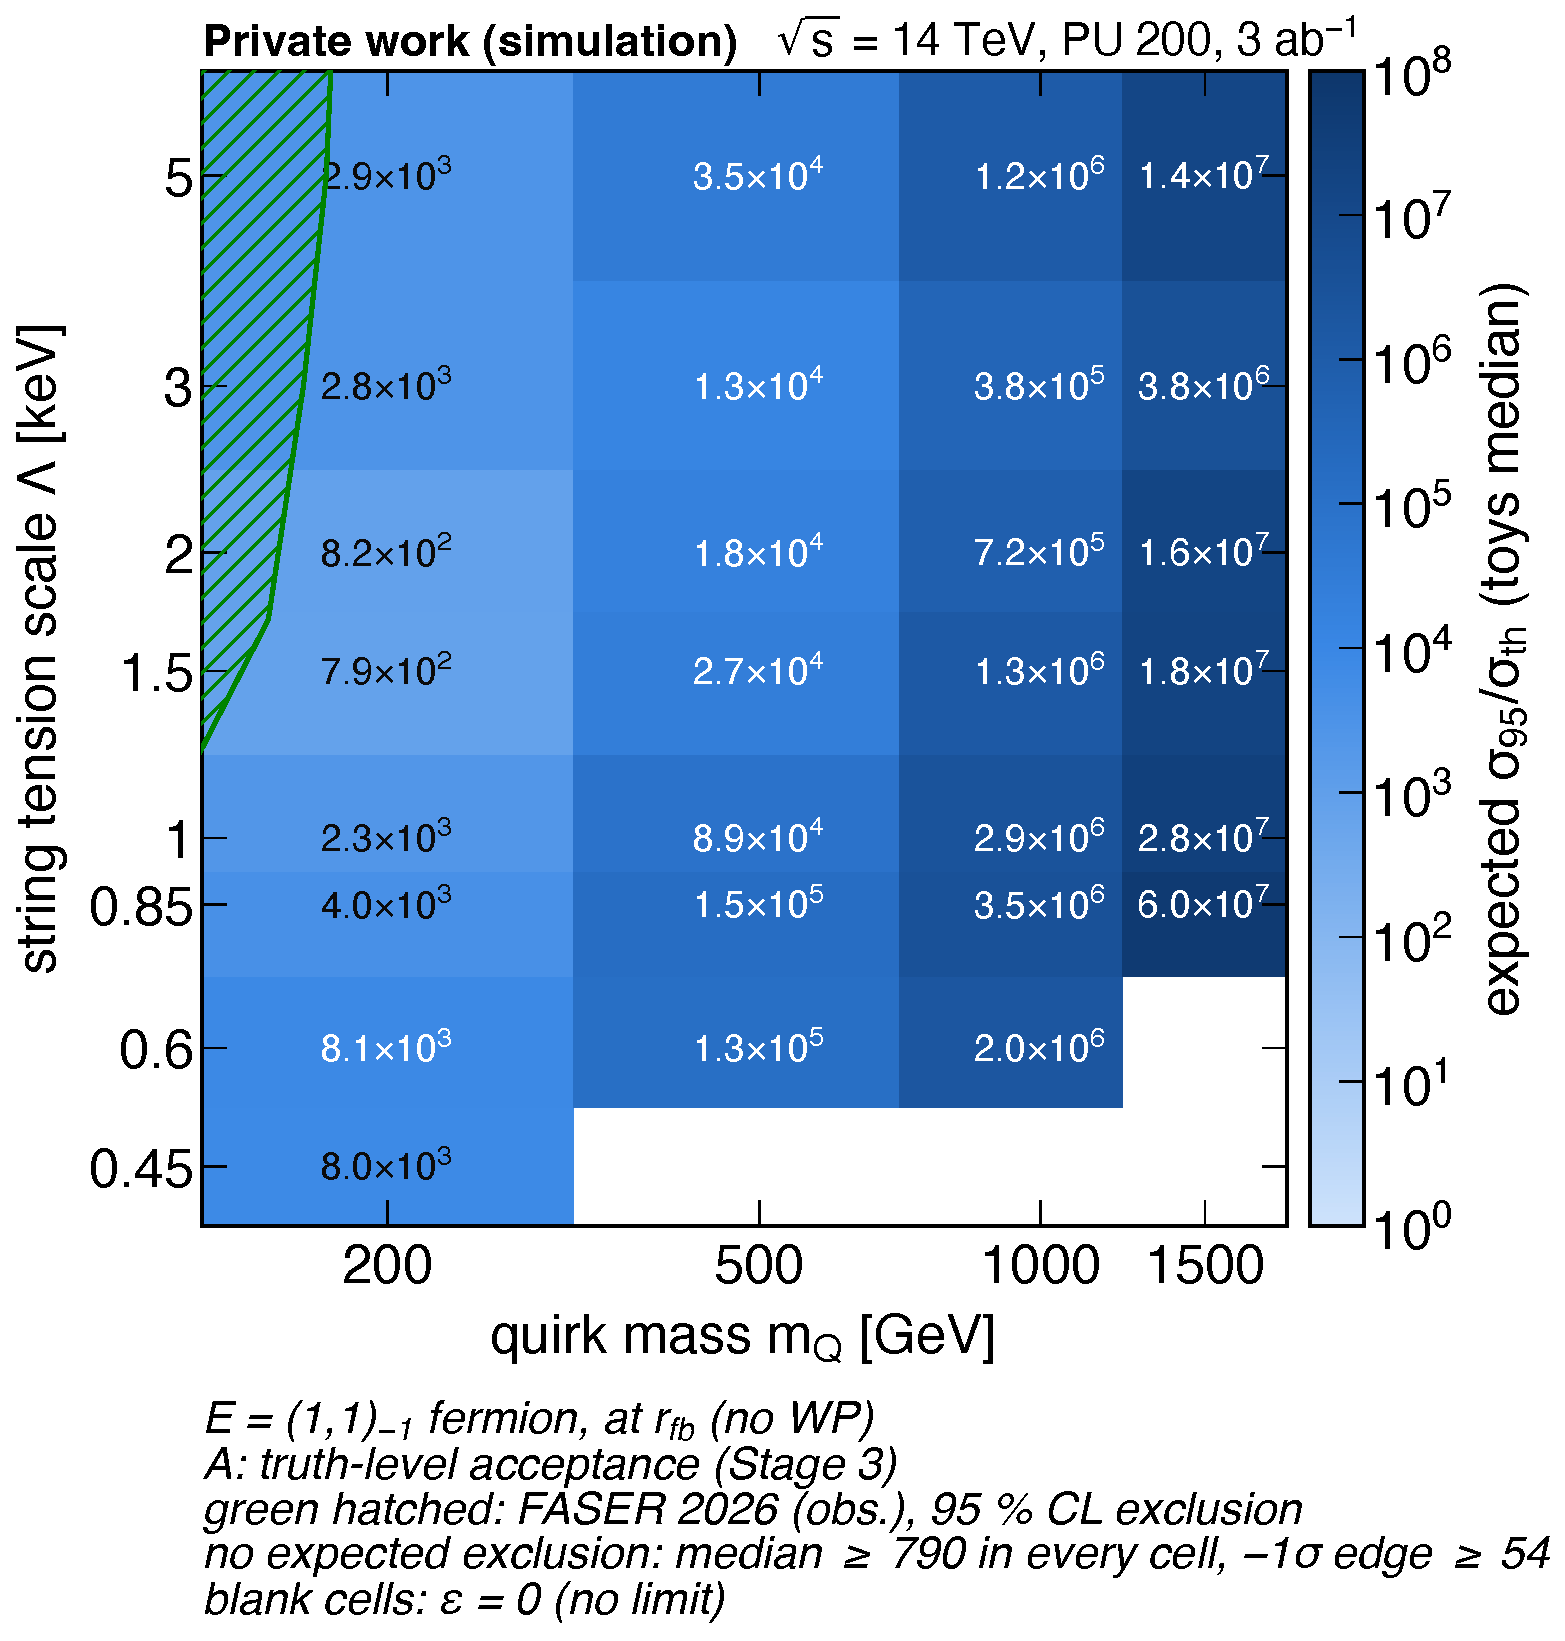
\includegraphics[height=0.44\linewidth]{figures/D7_exclusion_map.pdf}
\caption{Expected $\sigma_{95}/\sigma_{\rm norm}$ (toy median; labelled $\sigma_{95}/\sigma_{\rm th}$ in the figure) at the fallback selection on the
$(\mQ,\Lam)$ grid of the fermion $E$ (detector-level limit with truth-level acceptance; no working point). Every cell is
above one (median $\ge790$; the $-1\sigma$ toy edge $\ge54$), so nothing is excluded; blank cells have zero efficiency. The hatched region is the observed FASER exclusion~\cite{FASER:2026fsy}. Outside the plotted range lie
D0 ($\mQ<107\GeV$ at $\Lam=10\keV$--$1\MeV$~\cite{D0:2010kkd}), the Farina--Low benchmarks at $\Lam=1$ and
$100\eV$~\cite{Farina:2017cts}, and, as drawn by FASER, the heavy-stable-charged-particle recast
($\Lam\approx0.0024$--$0.22\keV$, $\mQ<685\GeV$), the monojet recast ($\mQ<57\GeV$) and the Evans--Luty out-of-time recast
($\Lam\approx0.0025$--$0.15\keV$, $\mQ<202\GeV$)~\cite{Evans:2018jmd}. The deep-rung background central values are zero-count
simulation bounds; the 31 fast-path points may overestimate $\Eff$ by up to $\approx1/0.87$
(Section~\ref{sec:results:eff}).}
\label{fig:excl}
\end{figure}
